
\documentclass[10pt,english]{article}
\usepackage[bottom=0.8in,margin=0.8in]{geometry}
\geometry{a4paper}
\usepackage[english]{babel}
\usepackage{indentfirst}
\selectlanguage{english}
\usepackage{multicol}
%\usepackage{varioref}% smart page, figure, table, and equation referencing
\usepackage[colorlinks]{hyperref}% hyperlinks [must be loaded after dropping]
\hypersetup{colorlinks,breaklinks,
citecolor = blue,
urlcolor=blue,
linkcolor=blue}
\usepackage[noabbrev]{cleveref}
\usepackage{float}

\usepackage{placeins}
\usepackage[utf8]{inputenc}

%Julia input
\usepackage[T1]{fontenc}
\usepackage{beramono}
\usepackage{listings}
\usepackage[usenames,dvipsnames]{xcolor}

\usepackage{amsmath}
\usepackage{xfrac}
\usepackage{gensymb}
\usepackage{graphicx}
\usepackage[colorinlistoftodos]{todonotes}
\usepackage{siunitx}
\usepackage{multirow}
\usepackage{subfig}
\usepackage{nomencl}
\makenomenclature

\definecolor{myred}{RGB}{200,50,50}
\definecolor{mycomments}{RGB}{75,100,175}

%%
%% Julia definition (c) 2014 Jubobs
%%
\lstdefinelanguage{Julia}%
{morekeywords={abstract,break,case,catch,const,continue,do,else,elseif,%
		end,export,false,for,function,immutable,import,importall,if,in,%
		macro,module,otherwise,quote,return,switch,true,try,type,typealias,%
		using,while},%
	sensitive=true,%
	alsoother={\$},%
	morecomment=[l]\#,%
	morecomment=[n]{\#=}{=\#},%
	morestring=[s]{"}{"},%
	morestring=[m]{'}{'},%
}[keywords,comments,strings]%

\lstset{%
	language       		 	  = Julia,
	basicstyle           	  = \ttfamily,
	tabsize				    	 =2,
	breaklines			 	 =true,
	keywordstyle     	 = \bfseries\color{myred},
	stringstyle      	 	  = \color{magenta},
	commentstyle    	= \color{mycomments},
	showstringspaces = false,
}
% End Julia input

\usepackage{graphicx}

\usepackage{amssymb}
\usepackage{authblk}
\graphicspath{{../figures/free_analytical/}} % allows figures to be placed in a different folder


\title{\vspace{-20pt}Analytical Derivation and Verification of Aircraft Transition and Climb Relations through Dynamic Optimization }
\author{Kevin R. Moore}
\affil{\vspace{-10pt}Brigham Young University}
\renewcommand\Authands{, }
\date{\today}

\begin{document}

\maketitle

\textbf{General aviation guidelines for takeoff are derived for relatively low thrust-to-weight aircraft and negate the transition between roll and steady climb.  Using dynamic optimization with full longitudinal flight dynamics shows that the transition period between roll and steady climb becomes significant above a thrust-to-weight ratio of 0.4.   Regardless of aircraft parameters, within feasible aircraft designs, the dominating constraint for the dynamic solution is the maximum lift coefficient throughout the rotation.  By using the maximum lift coefficient and calculating the centrifugal force due to thrust, gravity, lift, and drag, a simplified takeoff transition equation can be derived.  This simple equation is shown to account for the significant effects of takeoff transition for high thrust-to-weight aircraft and requires only one design evaluation.  }

\begin{multicols}{2}
\printnomenclature
\end{multicols}

\section{Motivation}

Electric propulsion has two main differences from fuel based propulsion: a high power-to-weight ratio and a low energy-to-weight ratio.  This enables aircraft designs that can meet takeoff requirements via high thrust at takeoff despite very highly loaded wings\cite{leap}.  In designing this type of aircraft, many of the assumptions made for general aircraft analysis no longer hold, such as a negligible transition between roll and climb at takeoff.  This paper showcases the need for including transition in the takeoff calculations for high power-to-weight aircraft.  Also included is the derivation of a simplified set of equations that describes the takeoff path including the effects of transition.  Results are verified through dynamic optimization.



\section{Dynamic Optimization}
To show the need for transition modeling in the takeoff path, I modeled the full aircraft longitudinal dynamics\cite{beard} including empirical stability and control derivatives\cite{aerosonde}.  I define the transition region as the time between zero pitch at the end of roll and the desired steady state flight path angle.  With the dynamic model, I performed numerical time integration using the DynamicalSystems.jl open source package, and specified 30 control points along the path.  At each of these control points, I changed thrust and elevator deflection, which then remained constant until the time integration progressed to the next control point.  This type of control can be classified as a shooting method.  To efficiently specify the control point inputs, I used SNOPT\cite{snopt}, a gradient based optimization package for large nonlinear constrained problems.  The objective and constraints were set up as follows:

\[
\begin{aligned}
& \text{minimize:} & & E = \sum{P \cdot V} \\
& \text{with respect to:} & & T, \delta_\text{elevator}\\
& \text{subject to:}
& &  \displaystyle P \leq P_{\text{max}}  \\
& & & \displaystyle V \geq V_{\text{min}}  \\
& & & \displaystyle h \geq h_{\text{ground}}  \\
& & & \displaystyle h_\text{end} \geq h_{\text{desired}}  \\
\end{aligned}
\]

\nomenclature{$P$}{Power (watts)}
\nomenclature{$V$}{Velocity (m/s)}
\nomenclature{$T$}{Thrust (N)}
\nomenclature{$V_{\text{min}}$}{Takeoff Speed}
\nomenclature{$h$}{Height (m)}

\vspace{10pt}
\noindent The aircraft initial conditions were set to start at the end of the roll state when the velocity achieved is the takeoff velocity but the pitch and flight path angle are still at zero degrees.

\Cref{f:dyanmic_path} shows the results of the optimization for a sweep of maximum power-to-weight.  Immediately, it can be seen that at and above a power-to-weight ratio of 6.8, the transition rotation becomes significant, taking as much or more than half of the path.  Power-to-weight was chosen as the defining metric in this case to better align with electric powered aircraft which are predominantly power constrained.  This means that the electric system would be able to produce much more thrust at a slower velocity as opposed to a faster velocity with the relation of P = TxV.  The approximate thrust-to-weight during the maneuver is also shown in \cref{f:dyanmic_path}.


\begin{figure}[H]
\centering
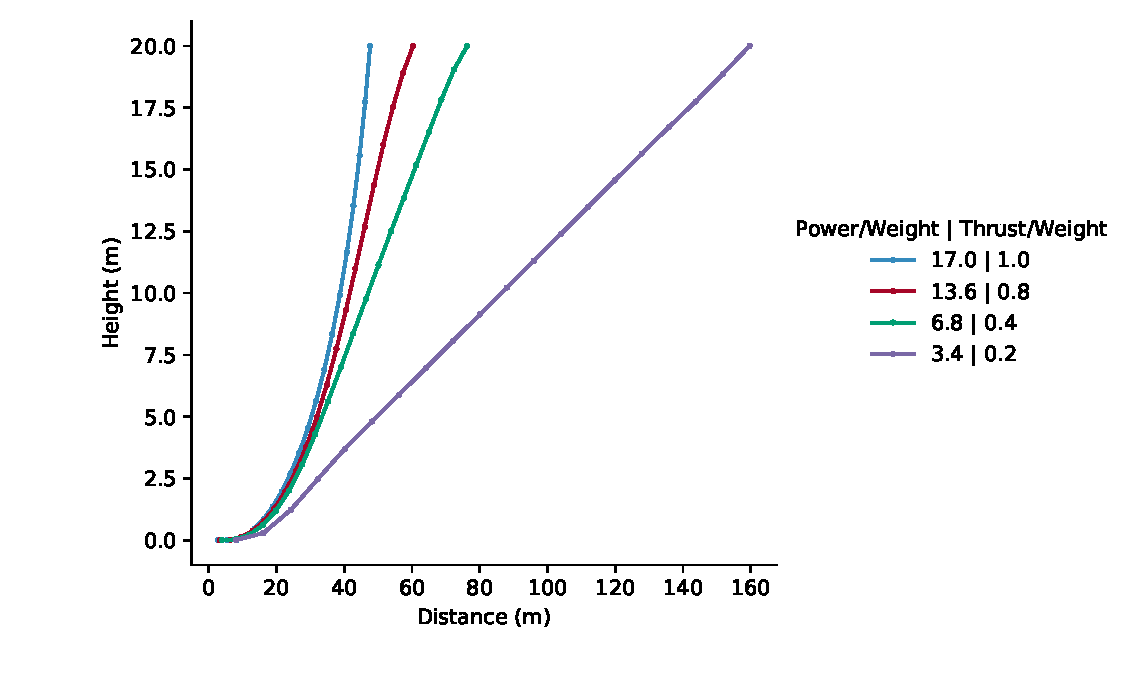
\includegraphics[trim={.0cm 0.5cm .0cm 0cm},clip,width=0.9\textwidth]{pn_pd}
\vspace{-5pt}
\caption{Optimal paths for a required final height of 20 meters shows the transition being significant above a power-to-weight of 6.8. Approximate thrust-to-weight is also shown for the maneuver.}
\label{f:dyanmic_path}
\end{figure}

Two notable and related results are that; First, above a certain amount of power, the minimum energy solution climb does not change with increasing power availability. Second, even for the lowest power-to-weight case, the steady state climb trajectory is not settled into until relatively late into the path.  Both of these results play into the same effect of the optimal control scheme modulating the flight velocity to build up momentum during the transition.  This momentum is used to temporarily increase the climb angle with little penalty in the power required.  For the high power cases, the tradeoff between momentum and power is balanced at around a power-to-weight of 13.6.  At this point, increasing the momentum with greater thrust during the transition does not decrease the total energy for the climb.  For the low power case, it is able to significantly increase the height in the first portion of the climb before settling into the shallower steady state climb angle.  \Cref{f:d_Va} shows this behavior with the velocity along the path quickly decreasing at the same positions as the heightened flight path angles.


\begin{figure}[H]
\centering
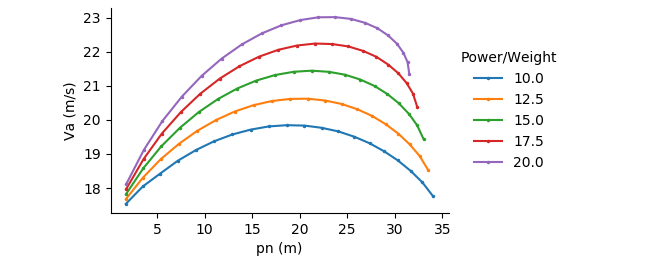
\includegraphics[trim={.0cm 0.5cm .0cm 0cm},clip,width=0.9\textwidth]{d_Va}
\vspace{-5pt}
\caption{Velocity buildup during the transition decreases the takeoff energy by balancing momentum buildup with power required. Approximate thrust-to-weight also shown for the maneuver.}
\label{f:d_Va}
\end{figure}

For all of the optimal paths, the main limiting factor despite changes in aircraft parameters, was the maximum lift coefficient during the rotation.  As the aircraft rotates, the maximum rate of rotation is limited by stall.  At the beginning of the path with the pitch at zero degrees, the pitch rate is very high.  Once the angle of attack is reached however, the pitch rate decreases to maintain the angle of attack at the maximum value.  This rate is modulated to keep the angle of attack at a maximum until the the optimal flight path angle (including momentum) is achieved.  After which, the angle of attack is modulated to stay at the optimal flight path angle for the available thrust and lift.

\begin{figure}[H]
\centering
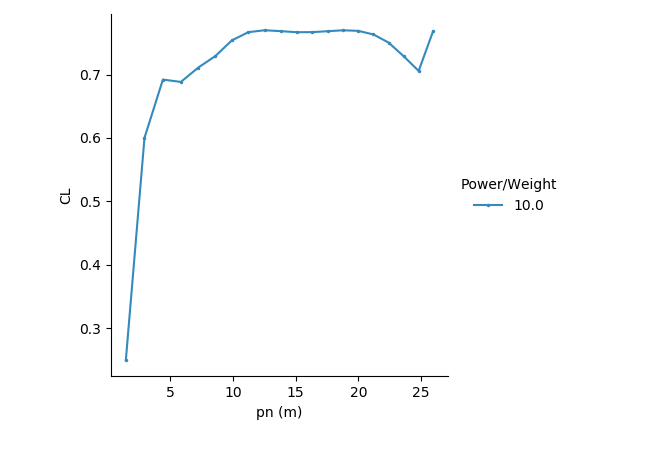
\includegraphics[trim={.0cm 0.5cm .0cm 0cm},clip,width=0.9\textwidth]{d_CL}
\vspace{-5pt}
\caption{Maximum CL for this aircraft is about 1.6, which is characteristic of the transition period for the range of power limits tested.}
\label{f:d_CL}
\end{figure}


\section{Steady Climb}
\label{s:steady_climb}

Before I define the derivation for a new analysis method for transition, I need to review the classic steady state climb relations.  Assuming acceleration in all directions is zero, the lift and net thrust must balance the gravity vector (see \cref{f:angles} for a definition of the coordinate system).

\begin{figure}[H]
\centering
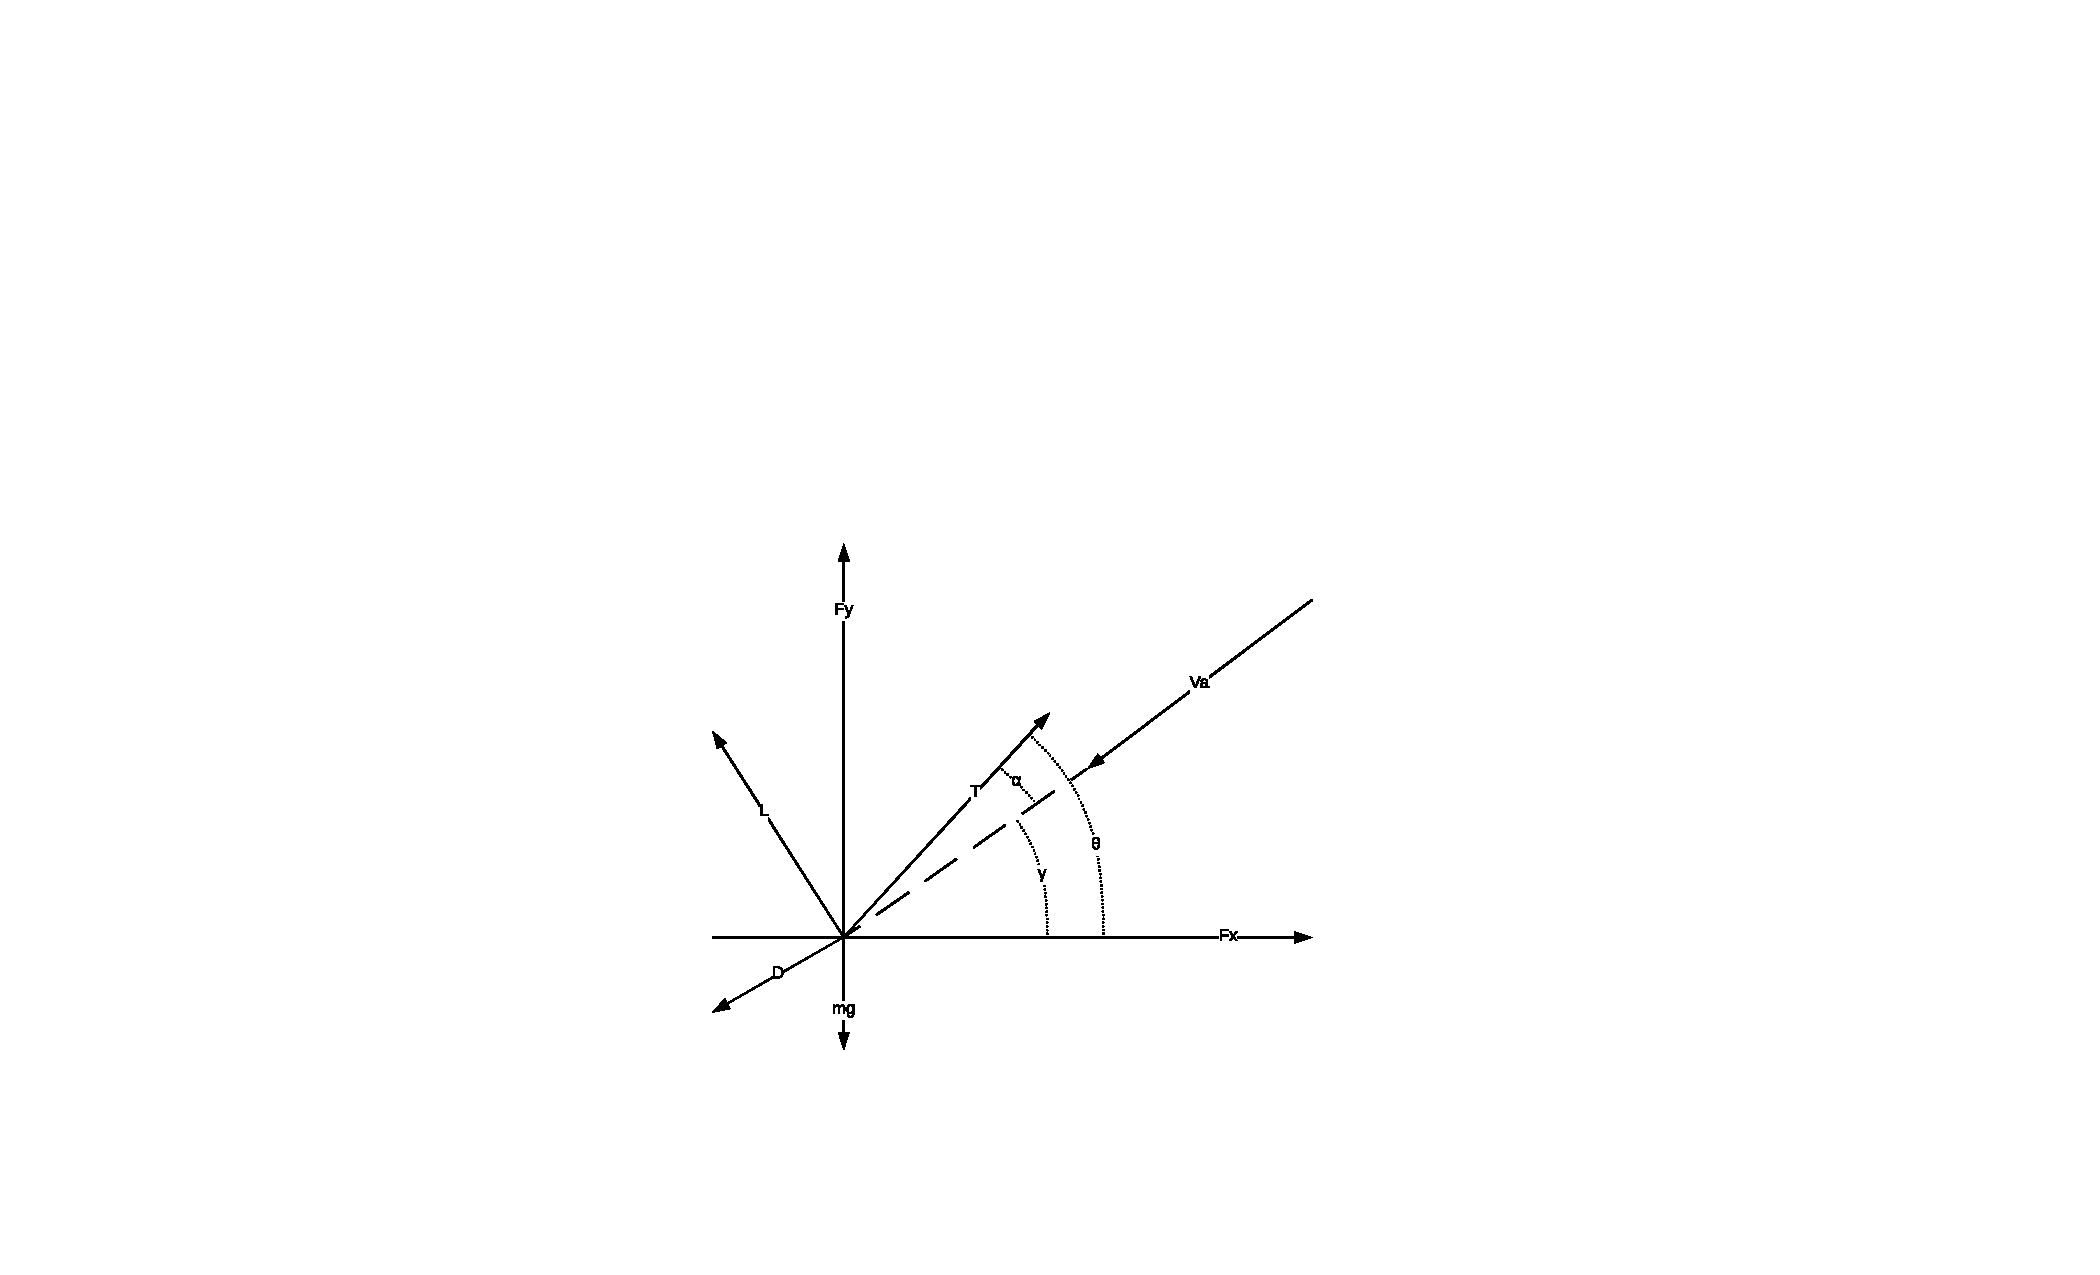
\includegraphics[trim={10cm 3.5cm 10cm 9cm},clip,width=0.9\textwidth]{Aircraft_Angles}
\vspace{-5pt}
\caption{Definition of relevant angles and forces.}
\label{f:angles}
\end{figure}




\begin{equation}
\label{eq:acceleration}
\dot{V_a} =\dot{V_x} = \dot{V_y} = 0
\end{equation}

\begin{equation}
\label{eq:lift}
L = m g  \cos(\gamma)
\end{equation}

\begin{equation}
\label{eq:thrust}
T-D = m g  \sin(\gamma)
\end{equation}

\vspace{10pt}

Using equation \ref{eq:thrust}, the flight path angle can be calculated as shown in equation \ref{eq:FPA}.  With the flight path angle, power, height, and thrust known, the total energy can be calculated as in equation \ref{eq:energy}.  These relations define the takeoff flight path after the transition and are an integral part of the new takeoff distance, power, and energy calculations.  Appendix A shows a more in depth tradeoff analysis including induced and viscous drag.

\begin{equation}
\label{eq:FPA}
\gamma = \sin^{-1}\Bigg(\frac{T-D}{mg}\Bigg)
\end{equation}

\begin{equation}
\label{eq:power}
P = T V_a
\end{equation}

\begin{equation}
\label{eq:energy}
E = \frac{T h }{\sin(\gamma)}
\end{equation}



\section{Transition}

Using Newton's second law (\cref{eq:newton}, we have an expression for the acceleration $\dot{V}$ as a function of force $F$ and mass $m$.  Next we formulate the aircraft body forces in \cref{eq:Fx,eq:Fy} including drag $D$, lift $L$, thrust $T$, flight path angle $\gamma$, pitch angle $\theta$, and gravity $g$.  For this simple example, we keep the thrust in line with the aircraft body axis and do not include the effects of angle of attack on thrust.  

\begin{equation}
\label{eq:newton}
\dot{V} = \frac{F}{m}
\end{equation}

\begin{equation}
\label{eq:Fx}
F_x = -D \cos(\gamma) - L \sin(\gamma) + T \cos(\theta)
\end{equation}

\begin{equation}
\label{eq:Fy}
F_y = L \cos(\gamma) - D \sin(\gamma) + T \sin(\theta) - m g
\end{equation}


Using similar triangles, we can use the alternative geometric form for the flight path angle to derive the expression for the rate change in flight path angle $\dot{\gamma}$ in \cref{eq:angledot1}.  Using the equations for force and acceleration in \cref{eq:newton,eq:Fx,eq:Fy} and inserting them into \cref{eq:angledot1}, we simplify the expression to \cref{eq:angledot}.  This final equation for the rate change in flight path angle is not easily integrated analytically due to the time derivative of the flight path angle and the nonlinearity of the inverse tangent, sines, and cosines.  If we assume a constant lift, airspeed, angle of attack, drag, and thrust during the maneuver, the equation becomes simple enough to be applied to a Taylor series expansion with three terms for the inverse tangent.  However, this method still results in an expression for the time integral that is several hundred terms in length.  If we could solve for the 

        \begin{equation}
\label{eq:angledot1}
\gamma = \tan^{-1} \Bigg(\frac{V_y}{V_x} \Bigg) => \dot{\gamma} = \tan^{-1} \Bigg(\frac{\dot{V_y}}{\dot{V_x}} \Bigg)
\end{equation}

        
        \begin{equation}
\label{eq:angledot}
\dot{\gamma} = \tan^{-1} \Bigg(\frac{L \cos(\gamma) - D \sin(\gamma) + T \sin(\theta)- m g}{-D \cos(\gamma) - L \sin(\gamma) + T \cos(\theta)}\Bigg)
\end{equation}

To fully characterize the transition path, one could use the x and y components of force and Newton's second law and numerically integrate to find the exact path over time.  However, this method cannot be reasonably integrated analytically due to the nonlinearity of the dynamic equations.  I will show this in the following example:

If we allow for acceleration in the x and y directions and apply Newton's second law as shown in equation \ref{eq:newton}, we can get relations for the x and y accelerations (including equations \ref{eq:Fx} and \ref{eq:Fy}).

\begin{equation}
\label{eq:newton}
\dot{V} = \frac{F_x}{m}
\end{equation}

\begin{equation}
\label{eq:Fx}
F_x = -D \cos(\gamma) - L \sin(\gamma) + T \cos(\theta)
\end{equation}

\begin{equation}
\label{eq:Fy}
F_y = L \cos(\gamma) - D \sin(\gamma) + T \sin(\theta) - m g
\end{equation}

\vspace{10pt}
\noindent If we also recall that the rate change of an angle is composed of the x and y rate changes, we derive equation \ref{eq:angledot}, which is the inverse tangent of the opposite and adjacent sides of the acceleration vector triangle.  This equation is not easily integrated due to the change in flight path angle, $\gamma$, with respect to time and the nonlinearity of the inverse tangent, sines, and cosines.  Assuming a constant lift, airspeed, angle of attack, drag, and thrust simplifies the equation enough to be applied to a Taylor series expansion of three terms for the inverse tangent.  However, this method still results in an expression for the time integral that is several hundred terms in length.

\begin{equation}
\label{eq:angledot}
\dot{\gamma} = \tan^{-1} \Bigg(\frac{L \cos(\gamma) - D \sin(\gamma) + T \sin(\theta)- m g}{-D \cos(\gamma) - L \sin(\gamma) + T \cos(\theta)}\Bigg)
\end{equation}

\vspace{10pt}
A simpler approach is to approximate the transition via a circular path and assume that the flight speed, lift, drag, angle of attack, and thrust are constant.  At the end of a 90 degree transition, the centrifugal force is equal to the force in the x-direction (equation \ref{eq:Fx}).  Using the dynamic equation for acceleration in a circular path allows us to calculate the circle's radius (equation \ref{eq:radius}).  With the radius known, the resulting x and y positions are calculated by equations \ref{eq:x} and \ref{eq:y}.  The final x and y positions can be calculated by using the steady state flight path angle from equation \ref{eq:FPA}.  With a constant thrust and velocity, the power calculation follows \ref{eq:power}, and the the time follows equation \ref{eq:t}. These assumptions performs well against a large range of flight path angles which will be shown in the following section.  Future work may include a transition between the $F_y$ and $F_x$ centrifugal forces in an elliptical path.

\begin{equation}
\label{eq:radius}
F_c = \frac{m V_a^2}{r} = F_x
\end{equation}

%                        \begin{equation}
%V_a = constant
%    \end{equation}
%
%                    \begin{equation}
%T = constant
%    \end{equation}

%                \begin{equation}
%\end{equation}

%|\dot{V_x}| = -|\dot{V_y}|
%    \end{equation}


\begin{equation}
\label{eq:x}
x = r \cos(\gamma)
\end{equation}

\begin{equation}
\label{eq:y}
y = r \sin(\gamma)
\end{equation}

\begin{equation}
\label{eq:t}
t = \frac{r \gamma}{V_a}
\end{equation}

\vspace{10pt}
Combining the steady climb path with the transition produces a new way to evaluate aircraft takeoff distance, energy, and rate of climb (when airspeed is included).  This new formulation shows, similarly to the dynamic optimization, that the transition period becomes a dominating factor as greater power is available to the aircraft.  This can be seen in \cref{f:analytical_takeoff}.   Also to note is the nearly negligible amount of transition for a low power-to-weight solution. Note that the thrust reported here is not the net thrust, and therefore the flight path angle will not be vertical due to the inclusion of drag for the highest thrust test shown.
\vspace{10pt}

\begin{figure}[H]
\centering
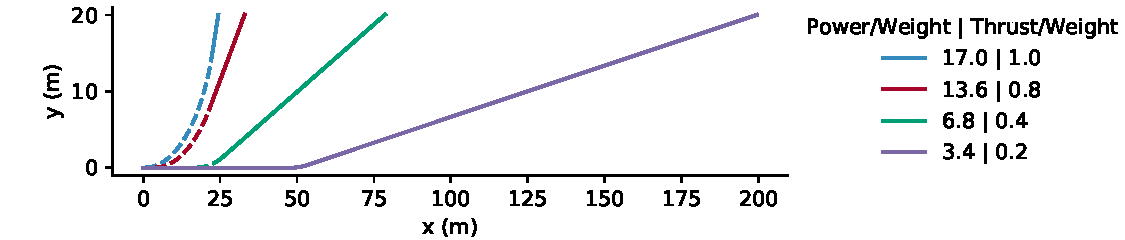
\includegraphics[trim={.6cm 0.0cm .1cm 0cm},clip,width=0.95\textwidth]{position}
%\vspace{-5pt}
\caption{Transition becomes increasingly dominant for higher power to weight.  Note that net thrust is not used here and drag decreases the flight path angle.}
\label{f:analytical_takeoff}
\end{figure}


\nomenclature{$\gamma$}{Flight path angle (rad)}
\nomenclature{$C_L$}{Aircraft wing lift coefficient}
\nomenclature{$E$}{Energy (joules)}
\nomenclature{$\alpha$}{Angle of attack (rad)}
\nomenclature{$\theta$}{Pitch (rad)}
\nomenclature{$L$}{Lift (N)}
\nomenclature{$D$}{Drag (N)}
\nomenclature{$F_x$}{Horizontal force (N)}
\nomenclature{$F_y$}{Vertical force (N)}
\nomenclature{$m$}{mass (kg)}
\nomenclature{$g$}{gravity (m/$\text{s}^2$)}
\nomenclature{$Va$}{Airspeed (m/s)}


\section{Comparison}

To fairly compare the two methods, dynamic optimization and analytical, I optimized the analytical path parameters of thrust, angle of attack, and flight speed while constraining the end of the path to be at the same position as the dynamic solution.  My objective was the same, minimize total energy, and the lift and drag were calculated using the same model as in the dynamic optimization.  \Cref{f:comparison} shows the comparison of the two solutions' paths.  It can be seen that the analytic equations slightly over-predict the rate of transition and under-predicts the flight path angle.  However, the analytical does not include the momentum buildup as explained previously which tends to sling-shot the aircraft into a temporarily steeper flight path angle.

\begin{figure}[H]
\centering
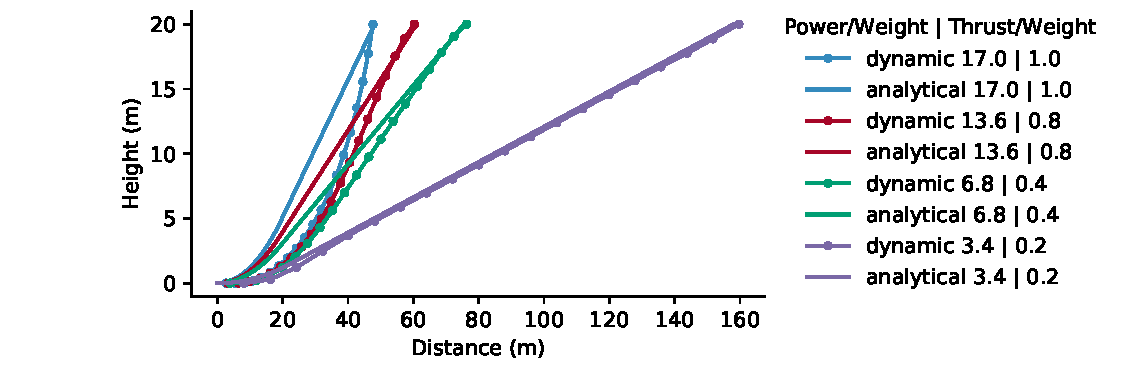
\includegraphics[trim={2.05cm 0.0cm .4cm 0cm},clip,width=0.95\textwidth]{pn_pd_compare}
\vspace{-5pt}
\caption{Paths match well considering the momentum buildup behavior of the dynamic solutions. Recall the flight path is unchanged above a power-to-weight of 13.6.}
\label{f:comparison}
\end{figure}

The greatest measure of accuracy for the analytical model is the energy required as shown in \cref{f:energy}.  Even though the paths are very close, the total energy for the maneuver differs by as much as 25\%.  This can be broken down into the thrust, velocity, and time.  

\begin{figure}[H]
\centering
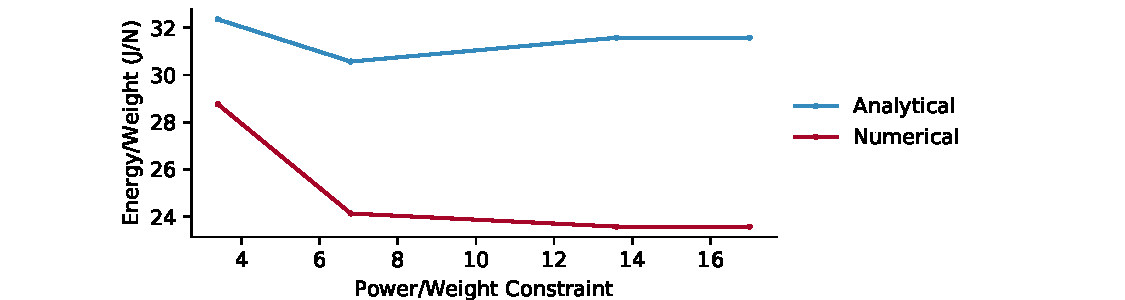
\includegraphics[trim={.7cm 0.0cm .7cm 0cm},clip,width=0.9\textwidth]{total_energy_compare}
\vspace{-5pt}
\caption{Total required energy matches fairly well considering the dynamic solutions' momentum buildup.}
\label{f:energy}
\end{figure}

\Cref{f:Va_compare} shows the analytical optimization choosing the lower bound on speed, the takeoff speed, across the board.  This is intuitive because it maximizes thrust for a constant power and in turns shortens the distance required for a given lift ceofficient.  

\begin{figure}[H]
\centering
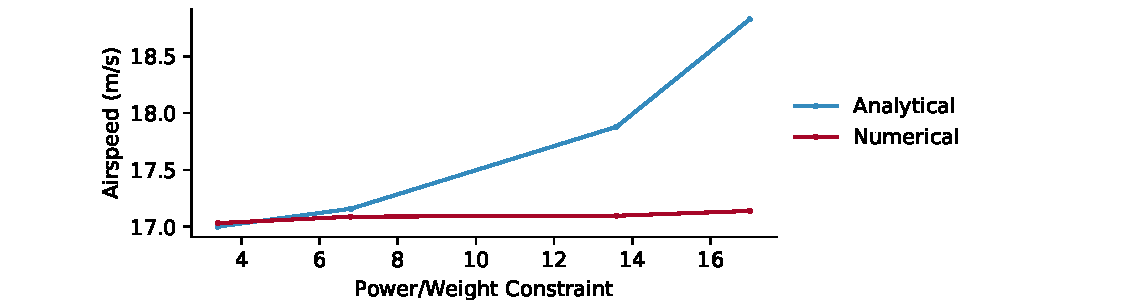
\includegraphics[trim={.7cm 0.0cm .7cm 0cm},clip,width=0.9\textwidth]{Va_compare}
\vspace{-5pt}
\caption{Analytical velocity at lower bound to maximize thrust for a constant power.}
\label{f:Va_compare}
\end{figure}

The analytical thrust (\cref{f:T_compare}) follows a similar trend as the dynamic results, but is higher due to not including momentum buildup.  

\begin{figure}[H]
\centering
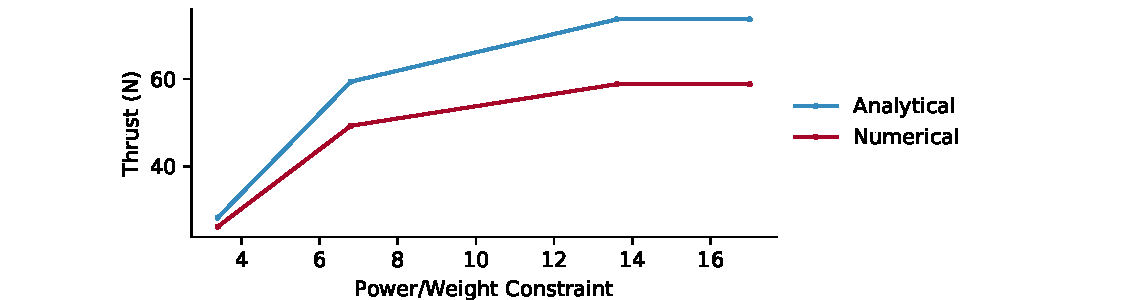
\includegraphics[trim={.7cm 0.0cm .7cm 0cm},clip,width=0.9\textwidth]{T_compare}
\vspace{-5pt}
\caption{Thrust for a given path higher due to the inability to harness momentum storage.}
\label{f:T_compare}
\end{figure}

The angle of attack (\cref{f:alpha_compare}) for the analytical is the balance between increasing lift, which decreases power for a given flight path angle (see Appendix A.),  and the increase in drag, which increases the total energy of the manuver.  

\begin{figure}[H]
\centering
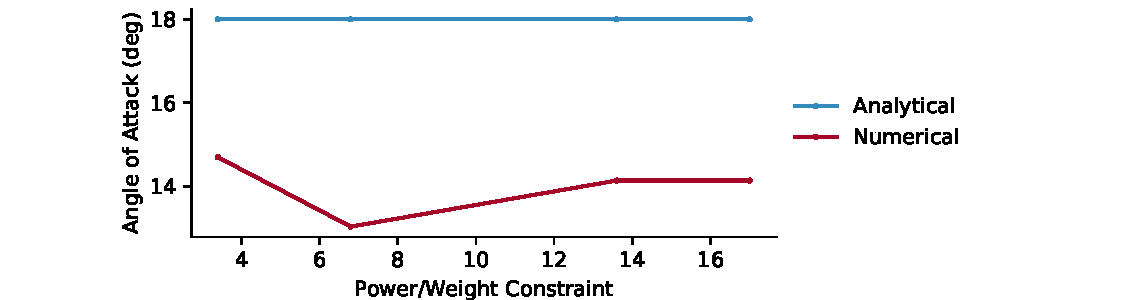
\includegraphics[trim={.7cm 0.0cm .7cm 0cm},clip,width=0.9\textwidth]{alpha_compare}
\vspace{-5pt}
\caption{Angle of attack near the upper bound of stall to tradeoff between lift (which decreases power for a given flight path angle see Appendix A.) and drag.}
\label{f:alpha_compare}
\end{figure}

Despite these differences, the time for the maneuver (\cref{f:t_compare}) matches very closely due to the semblance between paths as seen in \cref{f:comparison} and the relatively small deviation in airspeed. 


\begin{figure}[H]
\centering
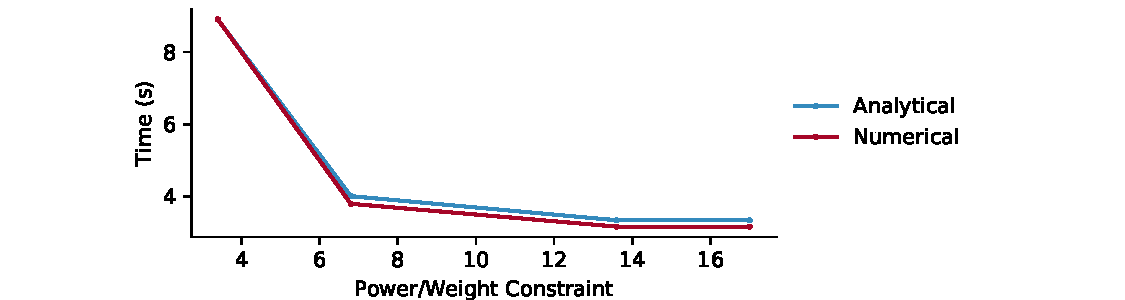
\includegraphics[trim={.7cm 0.0cm .7cm 0cm},clip,width=0.9\textwidth]{time_compare}
\vspace{-5pt}
\caption{Time for the maneuver matches quite closely due to a similar flight speed and distance.}
\label{f:t_compare}
\end{figure}

\section{Conclusions}
In this paper I derived and verified a new set of analysis equations for analytically characterizing the takeoff distance, time, power, and energy to achieve an altitude for a given aircraft mass.  I have shown that this type of simplified equation matches the path of a full longitudinal dynamic system when both are solved to minimize the takeoff energy for a given maximum power-to-weight ratio.  The dynamic optimization takes advantage of momentum buildup and is able to reduce the required thrust and in turn energy for the maneuver.  Despite this, the analytical derivation does account for the transition period of takeoff and requires only a single system design evaluation as opposed to several hundred for the dynamic optimization.  This difference will enable high power-to-weight aircraft multidisciplinary design optimization and account for the true takeoff distance, power, energy, and time with much more accuracy than current methods.  

If this analysis is to be continued, future work may include: validation against empirical data, constraining the dynamic optimization to stay at a specified speed, including a transition between y and x centrifugal forces in an ovalized path, and solving the full nonlinear differential equations to attain a more precise analytic function.

\bibliography{MainReferences}
\bibliographystyle{aiaa}

\section{Appendix A. Steady Climb Tradeoff Study}

Building on \cref{s:steady_climb}, I derive an equation for airspeed (equation \ref{e:Va}) composed of equations \ref{e:h_l} and \ref{e:L}.  This is important for calculating flight path angle, thrust, and power tradeoffs.  All of the values in equation \ref{e:Va} are known except the takeoff distance $d$ (the horizontal distance after roll to get to altitude).  The takeoff distance can be calculated by using the trigonometric relation in equation \ref{e:d1} with \ref{e:d0} to get the final equation \ref{e:d}.   Equations \ref{e:CD} and \ref{e:D} show the calculation of drag from lift and the parasitic drag.  This set of implicit equations must be iteratively solved to calculate the airspeed, $V_a$, for a given set of parameters.  However, the process is computationally inexpensive and gives significant insight into the tradeoffs involved with steady state climb.

\begin{equation}
\label{e:h_l}
\cos(\gamma) = \cos \Bigg(\tan^{-1}\bigg(\frac{h}{d}\bigg)\Bigg) = \frac{1}{\sqrt{1+(\frac{h}{d})^2}}
\end{equation}

\begin{equation}
\label{e:L}
L = C_L \frac{1}{2} \rho V_a^2 S_{\text{ref}} = m g \cos(\gamma)
\end{equation}

\begin{equation}
\label{e:Va}
V_a = \sqrt{\frac{2 m g}{C_L \rho S_{ref} \sqrt{(1+\frac{h}{d})^2}}}
\end{equation}

\begin{equation}
\label{e:d0}
\tan(\gamma) = \frac{h}{d} 
\end{equation}

\begin{equation}
\label{e:d1}
\tan \Bigg(\sin^{-1}\Bigg(\frac{T-D}{mg}\Bigg)\Bigg) = \sqrt{\bigg(\frac{m g}{T-D}\bigg)^2-1}
\end{equation}

\begin{equation}
\label{e:d}
d = h \sqrt{\bigg(\frac{m g}{T-D}\bigg)^2-1}
\end{equation}

\begin{equation}
\label{e:CD}
C_D = \frac{C_L^2}{\pi e_{wing} AR} + C_{Dp}
\end{equation}

\begin{equation}
\label{e:D}
D = C_D \frac{1}{2} \rho V_a^2 S_{ref}
\end{equation}

The tradeoff during climb can be summarized in the following three figures;  First, in \cref{f:TW_analytical}, the flight path angle is predominantly based on the aircraft thrust.  Increasing the lift coefficient decreases the net thrust some, but not in a significant manner with respect to the flight path angle.

\begin{figure}[H]
\centering
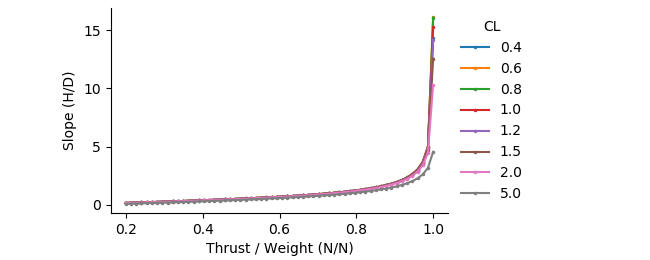
\includegraphics[trim={.0cm 0.0cm .0cm 0cm},clip,width=0.9\textwidth]{TW_analytical}
\vspace{-5pt}
\caption{Thrust is the major factor when determining the flight path angle.  Increasing lift coefficient increases the induced drag which decreases the net thrust.}
\label{f:TW_analytical}
\end{figure}

Second, in \cref{f:Power_dist_analytical}, as the lift coefficient increases, the power to fly a given flight path angle decreases substantially.  An example of this is if one were to fly at a flight path angle of 45 degrees.  It takes half the power to fly that path with a lift coefficient of 1.4 as opposed to a lift coefficient of 0.4.

\begin{figure}[H]
\centering
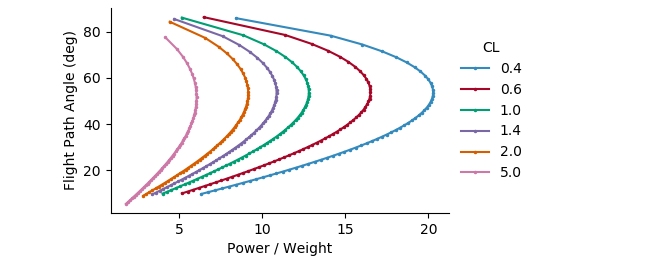
\includegraphics[trim={.0cm 0.0cm .0cm 0cm},clip,width=0.9\textwidth]{flight_angle_power_analytical}
\vspace{-5pt}
\caption{Lift coefficient plays a significant role in the power required for a given flight path angle.  Increasing from 0.4 to 1.4 halves the amount of power required for a 45 degree flight path angle.}
\label{f:Power_dist_analytical}
\end{figure}

Third, in \cref{f:t_compare}, as the lift coefficient increases, the total energy for the maneuver also increases.  This is due to the quadratic increase in induced drag.  However, if the drag does not increase quadratically by the use of high lift devices, powered or unpowered, there may be less of a penalty on the total energy.

\begin{figure}[H]
\centering
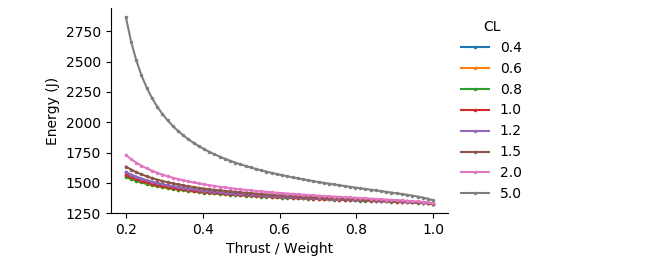
\includegraphics[trim={.0cm 0.0cm .0cm 0cm},clip,width=0.9\textwidth]{Energy_TW_analytical}
\vspace{-5pt}
\caption{Increasing lift coefficient decreases total energy for the climb until the maximum net power is achieved.  A lift coefficient of 0.6 is the best for the cases shown here.}
\label{f:t_compare}
\end{figure}

For aircraft design, these tradeoffs give insight into how one would design a propulsion system, or determine if optimization results are reasonable.  To decrease the power required for a given desired flight path angle, one must increase the lift coefficient, but to minimize the energy for the climb, one must decrease the drag until the maximum net power is achieved. 


\end{document}
